\documentclass{beamer}

\usepackage{pri}

\graphicspath{{./}{figures/}{figures/16-distributed-figs/}} 

\subtitle{Distributed Information Retrieval}

% http://grupoweb.upf.es/WRG/mir2ed/pdf/slides_chap10.pdf

\begin{document}

\maketitle

% ------------------------------------------------------------

\makeoutline

\begin{frame}
    \frametitle{Bibliography}
    \begin{block}{}
        \href{http://www.mir2ed.org/}{Ricardo Baeza-Yates,
            Berthier Ribeiro-Neto, Modern Information Retrieval, 2nd
            edtion}. Chapter 10.
    \end{block}
\end{frame}

\section{Introduction}

\begin{frame}
    \frametitle{Why Distributed IR?}
    
    \begin{itemize}
    \item The volume of online content today is staggering and it has been
        growing at an exponential rate
    \item On at a slightly smaller scale, the largest corporate intranets now
        contain several million Web pages
    \item As document collections grow larger, they become more expensive to
        manage
    \item In this scenario, it is necessary to consider alternative IR
        architectures and algorithms
    \item The application of parallelism and distributed computing can greatly
        enhance the ability to scale IR algorithms
    \end{itemize}
\end{frame}

\begin{frame}
    \frametitle{A Taxonomy of Distributed IR Systems}
    
    \begin{center}
        \begin{tabular}{|l|c|c|c|}\hline
          & & \multicolumn{2}{|c|}{Distributed} \\\cline{3-4}
          & Non-dist. & One system & Various systems \\\hline\hline
          Internal & standard & parallel & parallel \\\hline
          Local area & & cluster-based & local federated \\\hline
          Broadband & & distributed & fedarated \\\hline
        \end{tabular}
    \end{center}
\end{frame}

\section{Data Partitioning}

\subsection{Partitioning the Data}

\begin{frame}
    \frametitle{Document Partitioning}
    
    \begin{itemize}
    \item \emph{Document partitioning} slices the document-term matrix
        horizontally, dividing the documents among the subtasks
    \item The N documents in the collection are distributed across the P
        processors in the system
    \item During query processing, each parallel process evaluates the query on
        N/P documents
    \item The results from each of the sub-collections are combined into a
        final result list
    \end{itemize}
\end{frame}

\begin{frame}
    \frametitle{Term Partitioning}

    \begin{itemize}
    \item In \emph{term partitioning}, the matrix is sliced vertically
        \begin{itemize}
        \item It divides the indexing items among the P processors
        \end{itemize}
    \item In this way, the evaluation procedure for each document is spread
        over multiple processors
    \item Other possible partition strategies include divisions by
        \emph{language} or \emph{other intrinsic characteristics} of the data
    \item It may be the case that each independent search server is focused on
        a particular subject area
    \end{itemize}
\end{frame}

\begin{frame}
    \frametitle{Collection Partitioning}
    
    \begin{itemize}
    \item Available when the distributed system is centrally administered
    \item A first option is the \emph{replication of the collection} across all
        search servers
    \item The second option is \emph{random distribution of the documents}
        \begin{itemize}
        \item This is appropriate when a large document collection must be
            distributed for performance reasons
        \end{itemize}
    \item The final option is explicit \emph{semantic partitioning} of the
        documents
        \begin{itemize}
        \item Here the documents are often already organized into semantically
            meaningful collections
        \end{itemize}
    \item A broker routes queries to the search servers and balances the load
        on the servers
    \end{itemize}
\end{frame}

\subsection{Partitioning the Index}

\begin{frame}
    \frametitle{Inverted Index Partitioning}
    \begin{itemize}
    \item Document partitioning
        \begin{itemize}
        \item Logical
        \item Physical
        \end{itemize}
    \item Term partitioning
    \end{itemize}
\end{frame}

\begin{frame}
    \frametitle{Logical Document Partitioning}
    
    \begin{itemize}
    \item Uses the same inverted index as in the original algorithm
    \item Each dictionary entry includes P pointers into the corresponding
        inverted list
    \item The j-th pointer indexes the block of documents the sub-collection of
        the j-th processor
    \end{itemize}

    \centering
    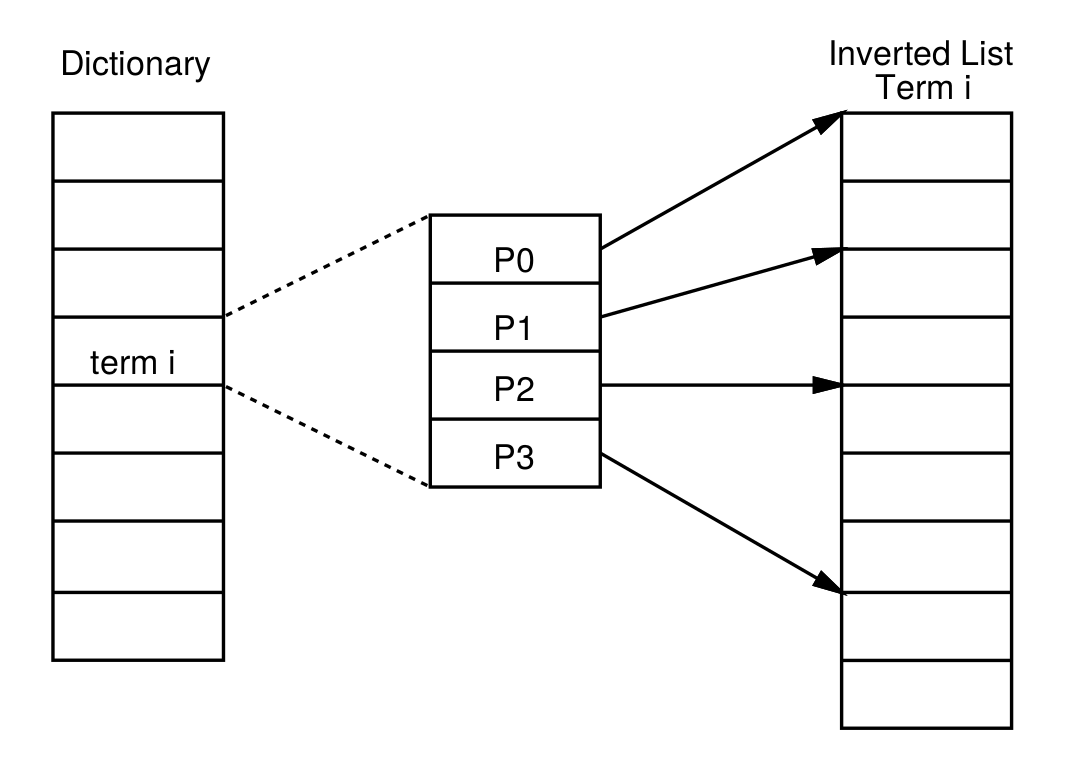
\includegraphics[width=.7\textwidth]{logicalpartitioning}
\end{frame}

\begin{frame}
    \frametitle{Physical Document Partitioning}
    \begin{itemize}
    \item Each sub-collection has its own inverted index and the processors
        share nothing during query evaluation
    \item Each processor evaluates the query on its portion of the document
        collection, producing a intermediate hit-list
    \item The P intermediate hit-lists can be merged efficiently using a binary
        heap-based priority queue
    \end{itemize}

    \centering
    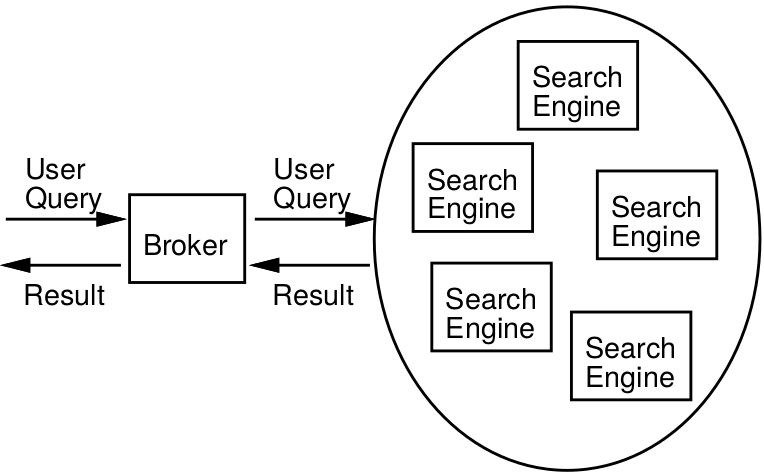
\includegraphics[width=.7\textwidth]{broker}
\end{frame}

\begin{frame}
    \frametitle{Physical Document Partitioning (cont.)}
    
    \begin{itemize}
    \item Each process may require \emph{global term statistics} in order to
        produce globally consistent document scores
    \item Two basic approaches:
        \begin{enumerate}
        \item Compute global term statistics at indexing time and store these
            statistics with each of the sub-collections
        \item Process the queries in two phases:
            \begin{enumerate}
            \item Term statistics from each of the processes are combined into
                global term statistics
            \item The broker distributes the query and global term statistics
                to the search processes
            \end{enumerate}
        \end{enumerate}
    \end{itemize}
\end{frame}

\begin{frame}
    \frametitle{Comparison}
    \begin{itemize}
    \item Logical document partitioning requires less communication than
        physical document partitioning
        \begin{itemize}
        \item Thus, it is likely to provide better overall performance
        \end{itemize}
    \item Physical document partitioning, on the other hand, offers more
        flexibility
        \begin{itemize}
        \item E.g., document partitions may be searched individually
        \end{itemize}
    \item The conversion of an existing IR system into a parallel system is
        simpler using physical document partitioning
    \end{itemize}
\end{frame}

\begin{frame}
    \frametitle{Term Partitioning}
    \begin{itemize}
    \item In term partitioning, the inverted lists are spread across the
        processors
    \item Each query is decomposed into items and each item is sent to the
        corresponding processor
    \item The processors create hit-lists with partial document scores and
        return them to the broker
    \item The broker then combines the hit-lists according
    \end{itemize}
\end{frame}

\begin{frame}
    \frametitle{Issues in Term Partitioning}
    \begin{itemize}
    \item The query load is not necessarily balanced, and thus part of the
        concurrency gains are lost
    \item Hence, the major goal is to partition the index such that:
        \begin{itemize}
        \item The number of contacted processors/servers is minimal; and
        \item Load is equally spread across all available processors/servers
        \end{itemize}
    \item We can use query logs to split the index vocabulary among the
        processors to achieve the goal above
    \end{itemize}
\end{frame}

\begin{frame}
    \frametitle{Overall Comparison}
    \begin{itemize}
    \item Document partitioning affords simpler inverted index construction and
        maintenance than term partitioning
    \item Assuming each processor has its own I/O channel and disks, document
        partitioning performs better
    \item When terms are uniformly distributed in user queries, term
        partitioning performs better
    \end{itemize}
\end{frame}

\section{Parallel IR}

% http://thedestination-vaibhav.blogspot.pt/2010/05/parallel-processing-sisdsimdmimdmisd.html
\begin{frame}
    \frametitle{Parallel Computing Architectures}
    
    \centering
    \begin{tabular}{cc}
      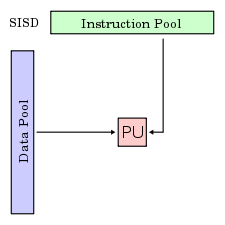
\includegraphics[width=.35\textwidth]{sisd} & 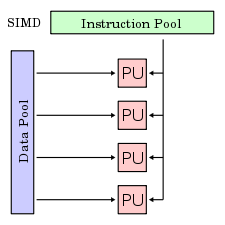
\includegraphics[width=.35\textwidth]{simd} \\
      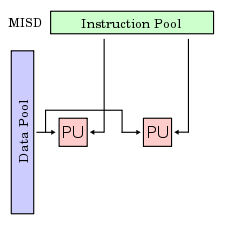
\includegraphics[width=.35\textwidth]{misd} & 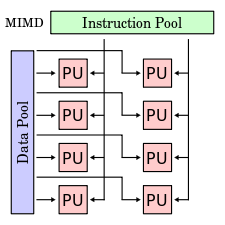
\includegraphics[width=.35\textwidth]{mimd} \\
    \end{tabular}
\end{frame}

\begin{frame}
    \frametitle{Parallel IR on MIMD Architectures}
    
    \centering
    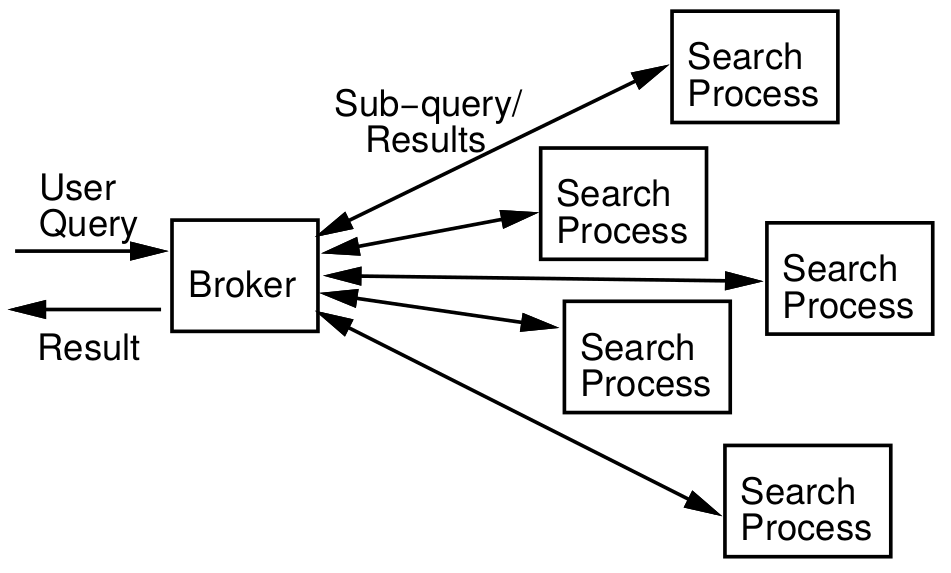
\includegraphics[width=.9\textwidth]{broker-mimd}
\end{frame}

\begin{frame}
    \frametitle{Issues with Parallel IR on MIMD}
    
    \begin{itemize}
    \item Care must be taken to \emph{properly balance the hardware resources}
        on the system
    \item Search processes running on the different processors can perform I/O
        and \emph{compete for disk access}
        \begin{itemize}
        \item A bottleneck at the disk will be disastrous for performance and
            could eliminate the throughput gains
        \end{itemize}
    \item In addition to adding more disks to the computer, the \emph{index
          data must be distributed} over the disks
        \begin{itemize}
        \item At one extreme, replicating the entire index on each disk
            eliminates disk contention at the cost of increased storage
            requirements and update complexity
        \item Alternatively, heavily accessed data can be replicated and less
            frequently accessed data can be distributed
        \end{itemize}
    \item Yet another approach is to \emph{install a disk array} and let the
        operating system handle partitioning the index
    \end{itemize}
\end{frame}

\section{Cluster-based IR}

\begin{frame}
    \frametitle{Cluster Computing}
    \begin{itemize}
    \item A \emph{cluster} of servers is a distributed system that has many
        computers, all physically close and usually connected through a fast
        local area network
        \begin{itemize}
        \item As local networks become faster, a cluster presents behavior that
            resembles that of a parallel machine
        \end{itemize}
    \item \emph{Load balancers} are special nodes that balance the load among
        different machines
    \end{itemize}
\end{frame}

\begin{frame}
    \frametitle{Cluster-based IR}
    \begin{itemize}
    \item To program a cluster, there are middleware software such as:
        \begin{itemize}
        \item MPI (Message Passing Interface)
        \item PVM (Parallel Virtual Machine)
        \end{itemize}
    \item Another possibility is the \emph{map-reduce} parallel computing
        paradigm
    \item Current research is focused on extending the power of the map-reduce
        paradigm
    \end{itemize}
\end{frame}

\begin{frame}
    \frametitle{Map-reduce}
    
    \centering
    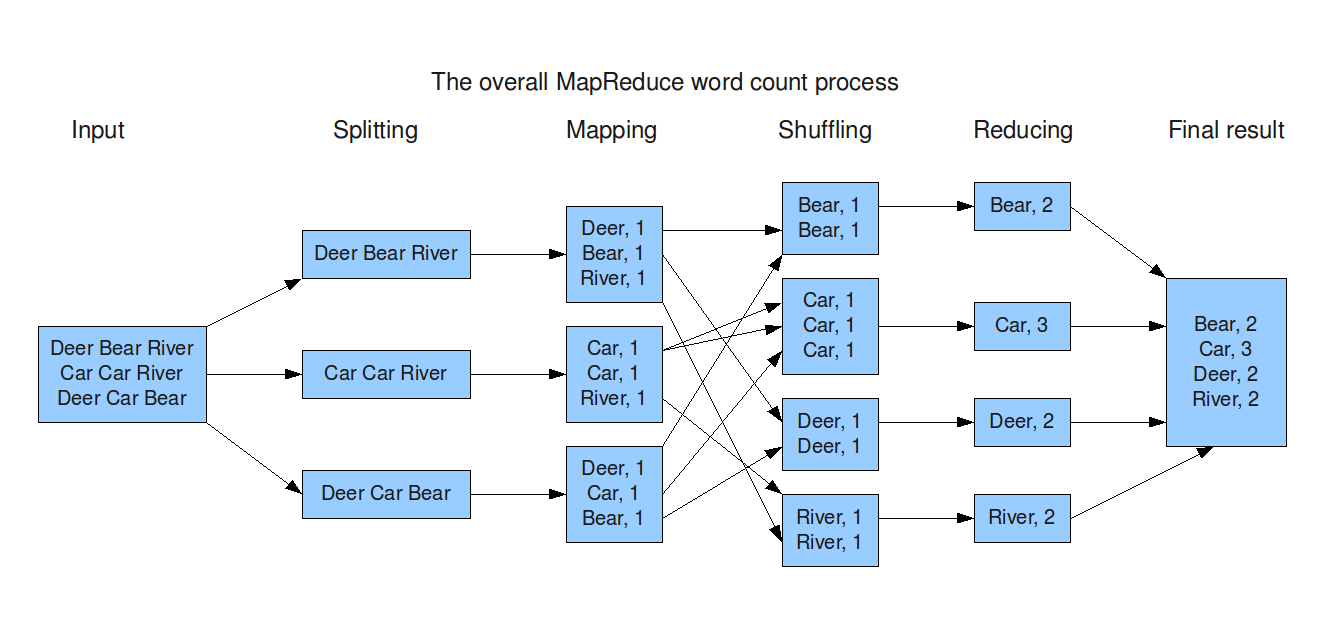
\includegraphics[width=\textwidth]{map-reduce}
\end{frame}

\section{Challenges in Distributed IR}

\subsection{Distributed Computing}

\begin{frame}
    \frametitle{Distributed Computing}
    \begin{itemize}
    \item Distributed computing uses multiple computers connected by a network
        to solve a single problem
        \begin{itemize}
        \item A distributed computing system can employ a heterogeneous
            collection of processors in the system
        \end{itemize}
    \item The cost of inter-processor communication is considerably higher in a
        distributed computing system
    \item In distributed computing each processor has its own local memory
    \end{itemize}
\end{frame}

\begin{frame}
    \frametitle{Key Issues}
    \begin{itemize}
    \item Four main issues:
        \begin{itemize}
        \item \emph{Partitioning} deals with data scalability and, in a large
            IR system, implies partitioning the document collection and the
            index
        \item \emph{Communication} deals with processing scalability, which in
            our case is query processing
        \item A system is \emph{dependable} if its operation is free of
            failures
        \item The \emph{external factors} are the external constraints on the
            system
        \end{itemize}
    \item Applications usually involve:
        \begin{itemize}
        \item Computation and data that can be split into coarse grained
            operations, and
        \item Relatively little communication is required between the
            operations
        \end{itemize}
    \item Parallel information retrieval based on document partitioning fits
        this profile well
    \end{itemize}
\end{frame}

\begin{frame}
    \frametitle{Modules of a distributed IR system}
    
    \centering
    \footnotesize
    \begin{tabular}{|c|ccc|}\hline
      & \multicolumn{3}{|c|}{Key Issues}\\\cline{2-4}
       &  & Dependability & External \\
      Module & Communication & (synchronization) & factors \\\hline\hline
      & & Partial indexing & Content growth \\
      Indexing & Reindexing & Updating & Content change \\
      & & Merging & Global statistics \\\hline
      &  & & Changing user needs \\
      Querying & Caching & Personalization & User base growth \\
      & Replication & Rank aggregation  & \\\hline
    \end{tabular}
\end{frame}

\subsection{Indexing}

\begin{frame}
    \frametitle{Indexing}
    \begin{itemize}
    \item One way to partition the index across the query processors is to
        consider the topics of the documents
        \begin{itemize}
        \item Routing the queries according to their topic involves identifying
            the topics of both documents and queries
        \item However, topic distribution might have a negative effect on the
            performance of the distributed retrieval system
        \end{itemize}
    \item Partitioning the index according to the language of queries is also a
        suitable approach
        \begin{itemize}
        \item A challenge in routing queries using language is the presence of
            multilingual documents such as in the Web
        \item In addition, queries can be multilingual, involving terms in
            different languages
        \end{itemize}
    \item So far, few papers suggest approaches to build an inverted index
        in a distributed fashion (comparatively)
    \end{itemize}
\end{frame}

\begin{frame}
    \frametitle{Dependability}
    
    \begin{itemize}
    \item If enough index servers fail, then the service as a whole also fails
    \item In some systems it is crucial to have the latest results for queries
        and content changes very often
        \begin{itemize}
        \item In this case, it is important that the index data available at a
            given moment reflects all the changes in a timely fashion
        \end{itemize}
    \item If a server of the system fails, it is impossible to recover the
        content of that server unless it is \emph{replicated}
        \begin{itemize}
        \item If this is not the case, then a possible inefficient way to
            recover is to \emph{rebuild the entire index}
        \item Another possibility would be to make the \emph{partitions
              partially overlapping}
        \item Document partitioned systems are more robust with respect to
            servers failures
        \end{itemize}
    \end{itemize}
\end{frame}

\begin{frame}
    \frametitle{Communication}
    
    \begin{itemize}
    \item The distributed \emph{merge operations} of the indexing process can
        impact the communication among servers
    \item Indexes are usually \emph{rebuilt from scratch after each update} of
        the underlying document collection
    \item This update operation usually requires locking the index,
        jeopardizing the whole system performance
    \item Terms that require frequent updates might be spread across the
        servers, thus amplifying the lockout effect
    \end{itemize}
\end{frame}

\begin{frame}
    \frametitle{External Factors}
    \begin{itemize}
    \item In a document partitioned IR system is necessary to compute values
        for some \emph{global parameters} such as
        \begin{itemize}
        \item the collection frequency, and
        \item the inverse document frequency of a term
        \end{itemize}
    \item There are two possible approaches:
        \begin{itemize}
        \item One can compute the final global parameter by aggregating all the
            local statistics available after the indexing phase
        \item The problem of computing global statistics can be moved to the
            system broker
        \end{itemize}
    \end{itemize}
\end{frame}

\subsection{Querying}

\begin{frame}{Query Processing}
    \begin{itemize}
    \item Resources to allocate to process a given query:
        \begin{itemize}
        \item A \emph{coordinator} makes decisions on how to route the queries
            to different parts of the system
        \item The \emph{query processors} hold index or document information
        \item \emph{Cache servers} can hold results for the most frequent or
            popular queries
            \begin{itemize}
            \item They can reduce query latency and load on servers
            \end{itemize}
        \end{itemize}
    \item One or more servers implement each of these components
        \begin{itemize}
        \item We can add more physical servers to increase the overall system
            capacity
        \end{itemize}
    \item As these servers can be in different physical locations, we call
        \emph{site} to each group of collocated servers
    \end{itemize}
\end{frame}

\begin{frame}
    \frametitle{Query Processing Architecture}
    
    \centering
    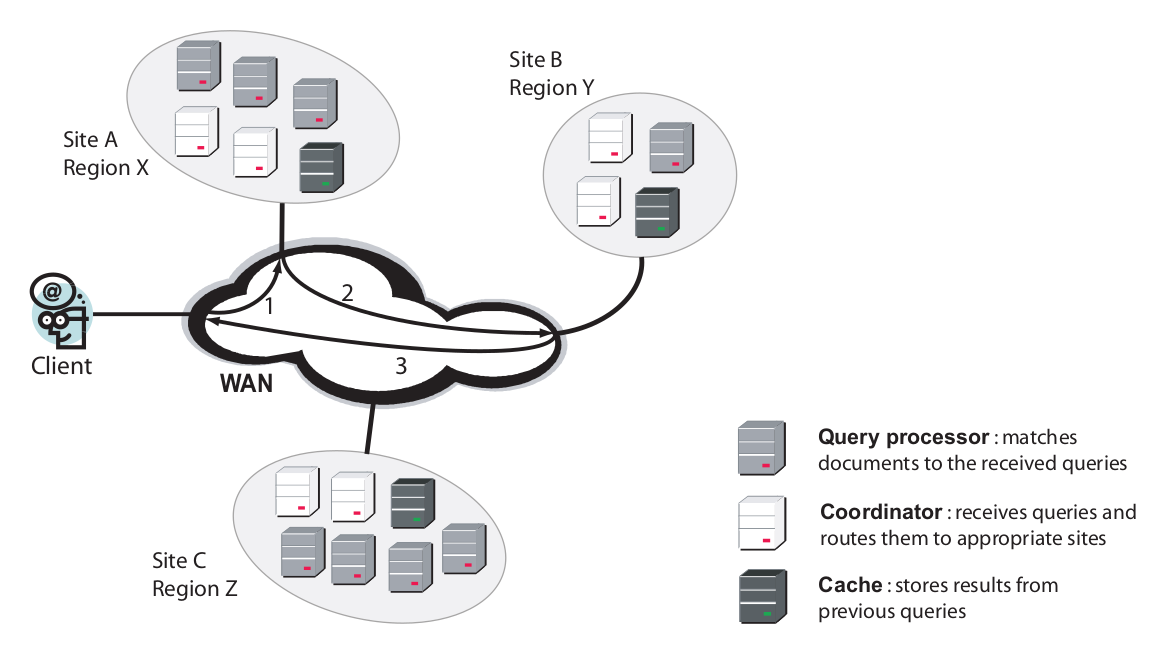
\includegraphics[width=\textwidth]{distributed}
\end{frame}

\begin{frame}
    \frametitle{Dependability}
    \begin{itemize}
    \item Due to the large amount of data they handle, it is challenging to
        determine good \emph{replication schemes}
        \begin{itemize}
        \item Having all query processors storing the same data, the system
            achieves the best availability level possible
        \item This is likely to impose a significant overhead
        \end{itemize}
    \item If a query processor is temporarily unavailable, we can serve
        \emph{cached results}
    \item \emph{Consistency} is also often a very important goal for online
        systems
        \begin{itemize}
        \item There are techniques from distributed algorithms to implement
            fault-tolerant services
        \end{itemize}
    \end{itemize}
\end{frame}

\begin{frame}
    \frametitle{Communication}
    \begin{itemize}
    \item If the index includes the \emph{position of terms}, the communication
        overhead between servers increases
        \begin{itemize}
        \item In such a case, the position information needs to be compressed
            efficiently
        \end{itemize}
    \item In the case of a document partitioned system, query processors send
        the query results to the coordinator
        \begin{itemize}
        \item The \emph{coordinator may become a bottleneck} while merging the
            results from a large number of query processors
        \end{itemize}
    \item Sometimes, the query processing involves \emph{adaptation of the
          search} results according to the interests of the user
        \begin{itemize}
        \item Each user profile represents a state, which must be the latest
            state and be consistent across replicas
        \end{itemize}
    \end{itemize}
\end{frame}

\begin{frame}
    \frametitle{External Factors}
    \begin{itemize}
    \item \emph{User behavior} is an external factor, which cannot be
        controlled by the IR system
        \begin{itemize}
        \item For example, the topics the users search for have slowly changed
            in the past
        \item Can also affect the performance of caching policies
        \end{itemize}
    \end{itemize}
\end{frame}

\section{Federated Search}

\begin{frame}
    \frametitle{Federated Search Engine}
    
    \begin{itemize}
    \item A federated search system relies on a collection of heterogeneous
        servers to answer user queries
    \end{itemize}
    \centering
    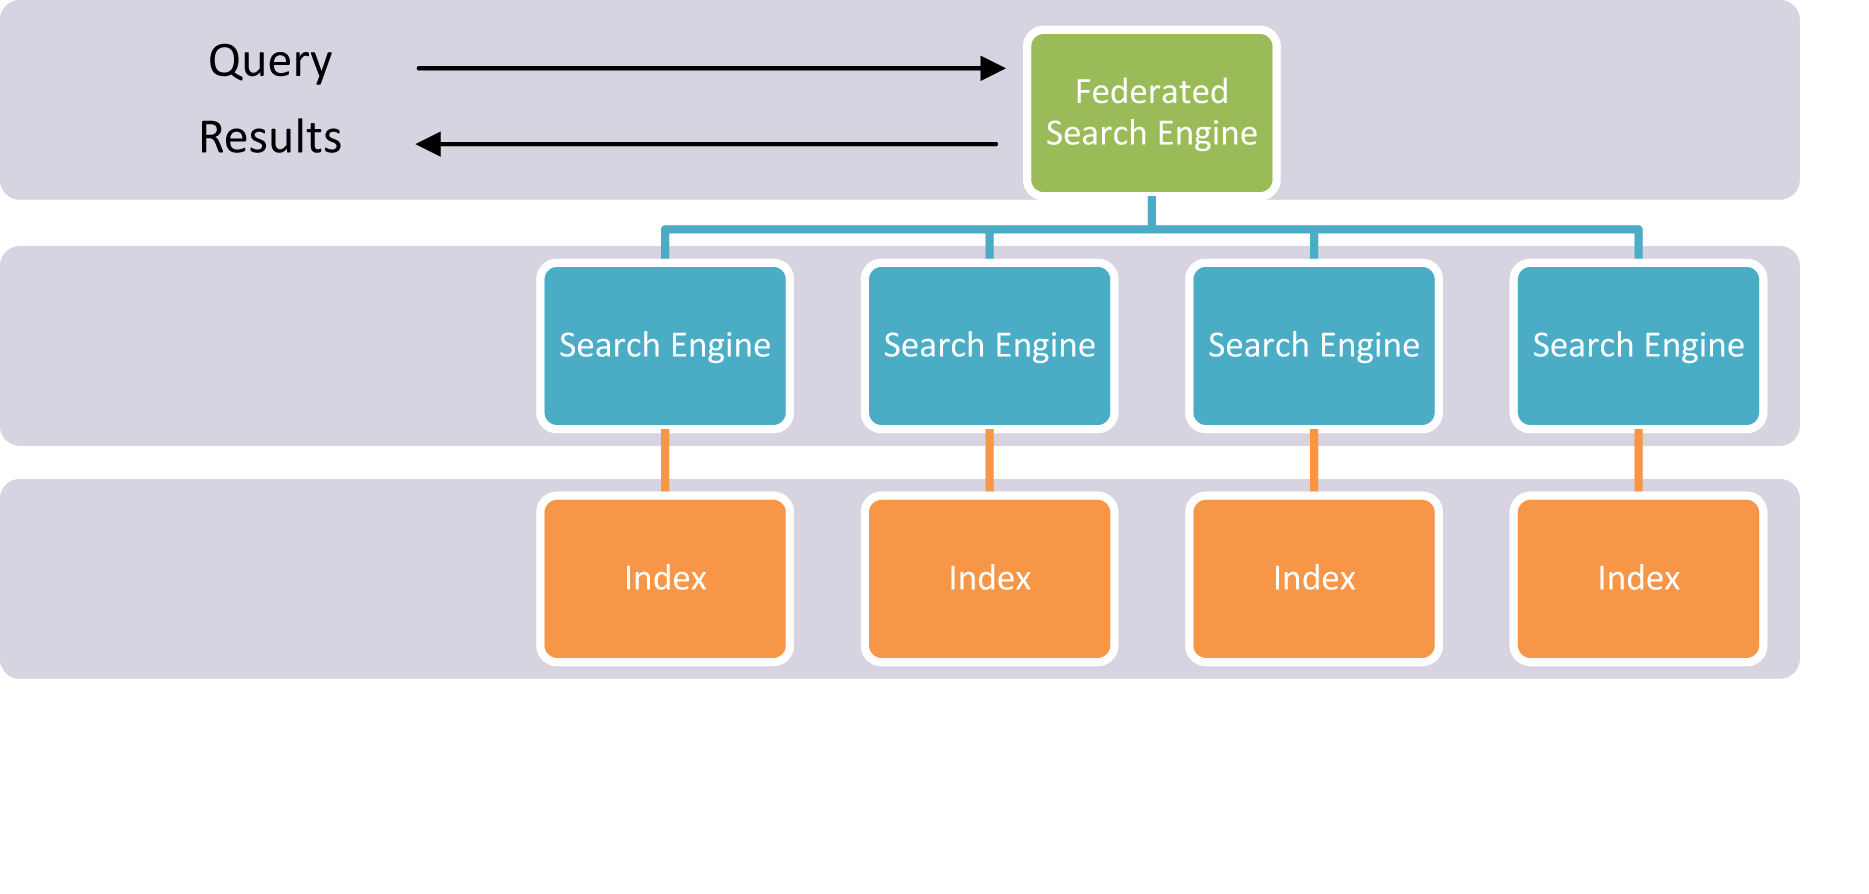
\includegraphics[width=\textwidth]{federated}
\end{frame}

\begin{frame}
    \frametitle{Engineering Issues}
    \begin{itemize}
    \item defining the \emph{search protocol} for transmitting requests and results,
        \begin{itemize}
        \item obtain information about a search sever
        \item submit a search request for one or more databases using a well
            defined query language
        \item receive search results in a well defined format
        \item retrieve items identified in the search results
        \item Standards: Z39.50, STARTS, OpenSearch, ...
        \end{itemize}
    \item designing a \emph{server} that can efficiently accept a request and initiate
        a thread
    \item designing a \emph{broker} that can submit asynchronous search
        requests to multiple servers and combine the results
    \end{itemize}
\end{frame}

\begin{frame}
    \frametitle{Algorithmic Issues}
    \begin{itemize}
    \item how to \emph{distribute documents} across the distributed search servers
    \item how to \emph{select which servers} should receive a particular query
    \item how to process the queries and \emph{combine the results} from the
        different servers
    \end{itemize}
\end{frame}

\begin{frame}
    \frametitle{How to merge the results?}
    \begin{itemize}
    \item The simplest approach is to combine the ranked hit-lists using round
        robin interleaving
    \item The most accurate technique for merging ranked hit-lists is to use
        accurate global term statistics
        \begin{itemize}
        \item Not always available
        \end{itemize}
    \item Use rank-merging techniques (we have seen those on a previous lesson)
    \end{itemize}
\end{frame}

\section{Retrieval in Peer-to-Peer Networks}

\begin{frame}
    \frametitle{Peer-to-Peer Networks}
    \begin{itemize}
    \item A \emph{peer} or node is an arbitrary computer which, when connected
        to the Internet, joins a peer-to-peer network, conforming a
        peer-to-peer (P2P) system
    \item IR algorithms can take advantage of resources distributed across
        Internet, in particular \emph{file sharing}
    \end{itemize}
\end{frame}

\begin{frame}[allowframebreaks]
    \frametitle{Retrieval in Peer-to-Peer Networks}
    \begin{itemize}
    \item Peer-level document collection descriptions can be used to identify
        nodes that can process the query
        \begin{itemize}
        \item These descriptions guide the peer-selection process and the
            document retrieval from the selected peers
        \item Resources are ranked by their likelihood to return relevant
            documents and top-ranked resources are selected
        \end{itemize}
    \item Document-level indexing approaches typically distribute the complete
        index in a structured P2P network
        \begin{itemize}
        \item This approach faces significant scalability problems caused by
            the high traffic costs
        \end{itemize}
\pagebreak
    \item Top-k query processing has been employed to solve the problem of
        extensive bandwidth consumption
        \begin{itemize}
        \item Terminate the processing of a query when the top- k results
            obtained so far are correct
        \end{itemize}
    \item Use hybrid index partitioning
        \begin{itemize}
        \item All peers are clustered in groups and the indexing technique
            employs term partitioning within the groups
        \end{itemize}
    \end{itemize}
\end{frame}

% ------------------------------------------------------------

\finalframe{Questions?}

\end{document}
